\documentclass[oneside, 11pt]{article}

\usepackage[T1]{fontenc}
\usepackage[utf8]{inputenc}
\usepackage[dutch]{babel}

\usepackage{fouriernc}
\usepackage[detect-all, load-configurations=binary,
            separate-uncertainty=true, per-mode=symbol,
            retain-explicit-plus, range-phrase={ tot }]{siunitx}

\usepackage{setspace}
\setstretch{1.2}

\setlength{\parskip}{\smallskipamount}
\setlength{\parindent}{0pt}

\usepackage{geometry}
\geometry{marginparwidth=0.5cm, verbose, a4paper, tmargin=3cm, bmargin=3cm, lmargin=2cm, rmargin=2cm}

\usepackage{float}

\usepackage[fleqn]{amsmath}
\numberwithin{equation}{section}
\numberwithin{figure}{section}

\usepackage{graphicx}
\graphicspath{{Figures/}}
\usepackage{subfig}

\usepackage{tikz}
\usetikzlibrary{plotmarks}

\usepackage{fancyhdr}
\pagestyle{fancy}
\fancyhf{}
\rhead{\thepage}
\renewcommand{\footrulewidth}{0pt}
\renewcommand{\headrulewidth}{0pt}

\usepackage{relsize}
\usepackage{xspace}
\usepackage{url}

\newcommand{\figref}[1]{Figuur~\ref{#1}}

\newcommand{\hisparc}{\textsmaller{HiSPARC}\xspace}
\newcommand{\kascade}{\textsmaller{KASCADE}\xspace}
\newcommand{\sapphire}{\textsmaller{SAPPHiRE}\xspace}
\newcommand{\jsparc}{\textsmaller{jSparc}\xspace}
\newcommand{\hdf}{\textsmaller{HDF5}\xspace}
\newcommand{\aires}{\textsmaller{AIRES}\xspace}
\newcommand{\csv}{\textsmaller{CSV}\xspace}
\newcommand{\python}{\textsmaller{PYTHON}\xspace}
\newcommand{\corsika}{\textsmaller{CORSIKA}\xspace}
\newcommand{\labview}{\textsmaller{LabVIEW}\xspace}
\newcommand{\daq}{\textsmaller{DAQ}\xspace}
\newcommand{\adc}{\textsmaller{ADC}\xspace}
\newcommand{\adcs}{\textsmaller{ADC}s\xspace}
\newcommand{\Adcs}{A\textsmaller{DC}s\xspace}
\newcommand{\hi}{\textsc{h i}\xspace}
\newcommand{\hii}{\textsc{h ii}\xspace}
\newcommand{\mip}{\textsmaller{MIP}\xspace}
\newcommand{\hisparcii}{\textsmaller{HiSPARC II}\xspace}
\newcommand{\hisparciii}{\textsmaller{HiSPARC III}\xspace}
\newcommand{\pmt}{\textsmaller{PMT}\xspace}
\newcommand{\pmts}{\textsmaller{PMT}s\xspace}

\DeclareSIUnit{\electronvolt}{\ensuremath{\mathrm{e\!\!\:V}}}

\DeclareSIUnit{\unitsigma}{\ensuremath{\sigma}}
\DeclareSIUnit{\mip}{\textsmaller{MIP}}
\DeclareSIUnit{\adc}{\textsmaller{ADC}}

\DeclareSIUnit{\gauss}{G}
\DeclareSIUnit{\parsec}{pc}
\DeclareSIUnit{\year}{yr}



\title{Weerstation met Arduino}
\author{C.G.N. van Veen}
\docweerstation{1}{WA}
\version{1.2 05-2015}

\begin{document}

\maketitle

\section{Weerstation}

\paragraph{Inleiding}
Naast het meten aan kosmische straling met het \hisparc meetstation kunnen  
leerlingen het \hisparc station uitbreiden met een weerstation gemaakt met Arduino.
Dit weerstation heeft als voordeel dat leerlingen dit zelf kunnen bouwen, aanpassen,
programmeren, wind- en water dichtmaken in een box en plaatsen bij het station.
Zo kunnen zij metingen van luchtdruk, buitentemperatuur en temperatuur van de 
detectorplaten meten en correleren met gemeten kosmische straling. Daarnaast 
kan het station uitgebreid worden met andere sensoren zoals UV-index, bliksem, 
regen en windsensoren.

\begin{figure}
    \centering
    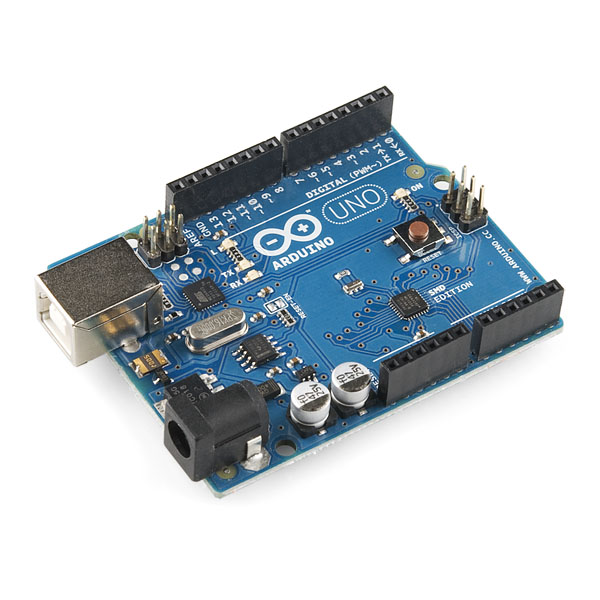
\includegraphics[scale=1.2]{Arduino}
    \caption{Arduino Uno R3, basis voor het weerstation}
   \label{fig:Arduino}
\end{figure}

\paragraph{Benodigdheden}
Het weerstation kan met meer sensoren uitgerust worden dan hier genoemd.
Het basis weerstation (luchtdruk, temperatuur en luchtvochtigheid) waar wij mee
getest hebben heeft de volgende onderdelen nodig: \\
\begin{itemize}
    \item Arduino Uno R3 (of elke andere Arduino)
    \item USB kabel
    \item DTH22 (of DTH11) luchtvochtigheid
    \item BMP085 luchtdruksensor
    \item DS18B20 digitale temperatuursensor (2 of 4x)
    \item arduino software
\end{itemize}

Andere sensoren zoals een bliksemdetector (AS3935) zijn tot op heden
niet getest, maar geven leerlingen een extra onderzoek
mogelijkheid(namelijk de correlatie tussen bliksem en kosmische
straling.)

\section{Arduino}

\subsection{Werking van Arduino}

Een Arduino is een microcontroller met een ATMEGA-328 chip die bestaat
uit een printplaatje met een aantal digitale en analoge ingangen, waar
bijvoorbeeld sensoren op aangesloten kunnen worden, zie
\figref{fig:Arduino}. Data van de sensoren kan via usb of draadloos (wat
wij gaan doen) ingelezen worden in de Arduino software of met een ander
programma. Deze software is vrij te downloaden van
\url{http://arduino.cc}. Als u al ervaring heeft met Arduino zal het
aansluiten van sensoren redelijk eenvoudig zijn. Als er nog geen
ervaring is met Arduino zijn er op het internet een aantal handleidingen
en tutorials beschikbaar evenals Arduino starterkits. Het wordt
aanbevolen om eerst een aantal basisschakelingen te maken met Arduino.
Voorbeelden van handleidingen zijn te vinden  op \url{http://arduino.cc}
of \url{http://arduino.nu}

Zoals in \figref{fig:Arduino} te zien is zijn er zes analoge ingangen
A0-A5 en zes digitale ingangen (pin 2 t/m 7). Voor het basis weerstation
zullen we van beide twee ingangen gebruiken. Het voordeel van digitale
ingangen is dat zij meerdere waarden kunnen verwerken. Er kunnen dus
meerdere digitale temperatuursensoren (DS18B20) op één digitale ingang
aangesloten worden.

De Arduino software heeft een aantal voorbeelden, die de gebruiker snel
een aantal zaken leert. Door de voorbeelden te bestuderen kun je
redelijk snel programmatuur onder de knie krijgen. Voor ons is het
belangrijk dat we Arduino gebruiken om sensorwaarden uit te lezen. In
de Arduino software is dan het voorbeeld:
\url{/Tutorial/AnalogReadSerial} erg belangrijk. Het voorbeeldprogramma
"AnalogReadSerial" bijvoorbeeld staat onder \emph{file / tools /examples /
Basics}. Zie \figref{fig:Arduino_example}.  

Sluit de Arduino aan met de USB kabel op de pc. Controleer dat de
Arduino software de Arduino vindt. Kijk hiertoe in het menu: \emph{
Tools / Serial Port }. Meestal vindt de software de usb poort vanzelf.
Zie \figref{fig:Arduino_serial}.

\begin{figure}
    \centering
    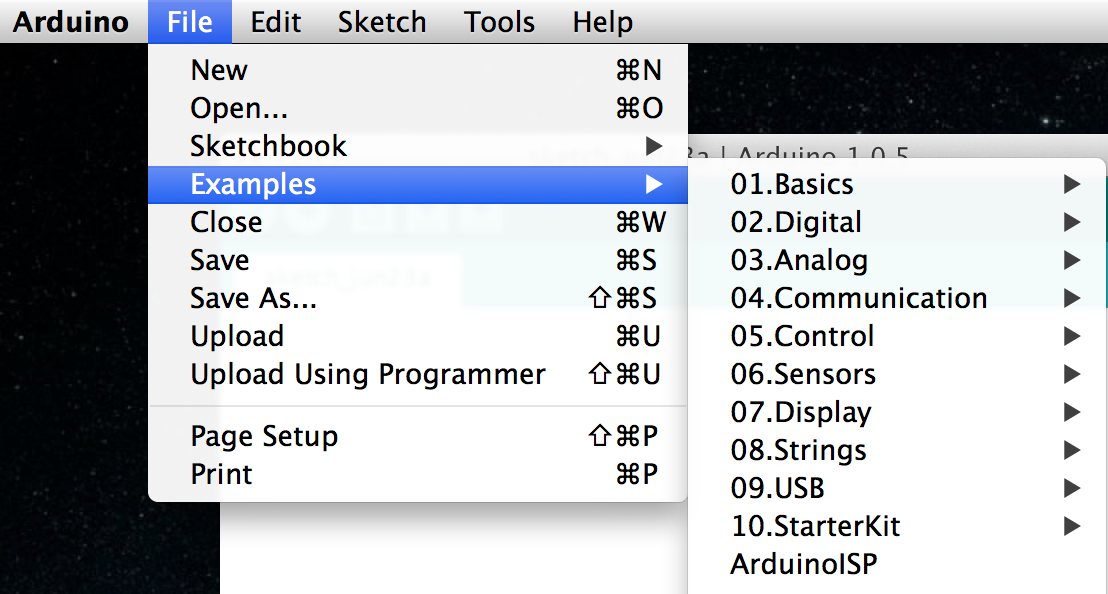
\includegraphics[scale=0.4]{Arduino_example}
    \caption{Arduino Software, voorbeeld programma's}
   \label{fig:Arduino_example}
\end{figure}

\begin{figure}
    \centering
    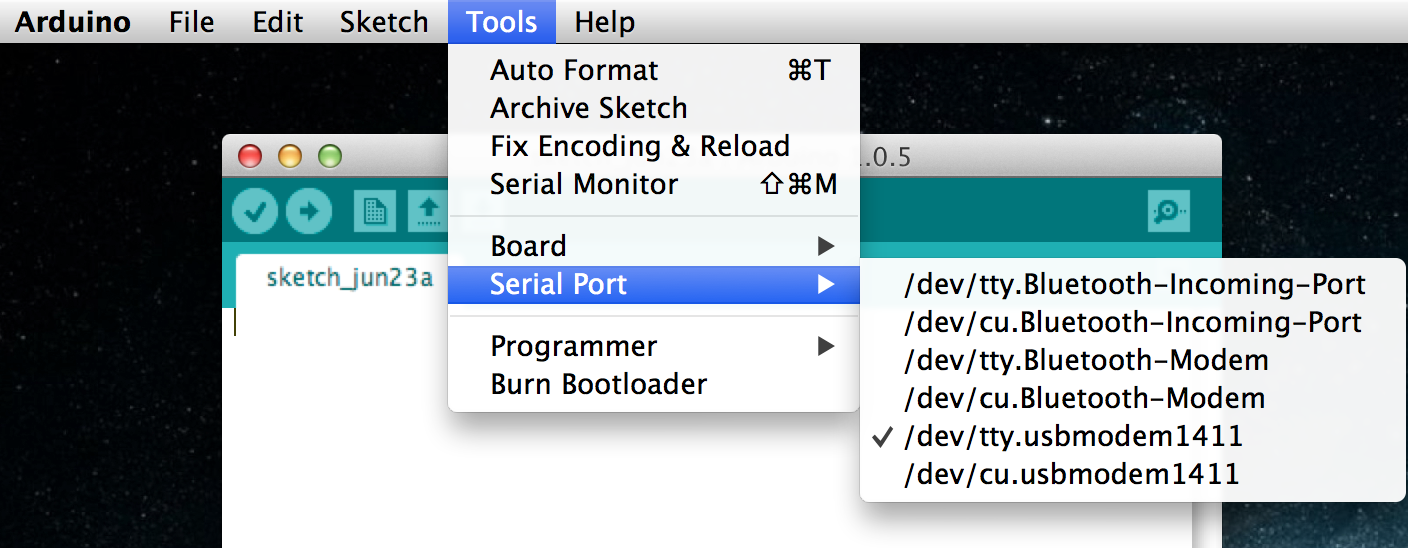
\includegraphics[scale=0.6]{Arduino_serial}
    \caption{Arduino Software, USB poort is gevonden door de software}
    \label{fig:Arduino_serial}
\end{figure}


\subsection{Programmeren in Arduino}

Het programmeren in Arduino is relatief eenvoudig. Een programma of
`sketch' bevat een header en twee \emph{void} onderdelen. In de header
worden libraries aangeroepen, elke library een bepaalde
functionaliteit, bijv. een library die de ijking van een sensor bevat.
Daarnaast kunnen in de header datapins en variabelen gedefinieerd worden
en onderdelen van libraries aangeroepen worden. In \emph{void setup}
kunnen ook variabelen gedefinieerd en kunnen libraries aangeroepen, ook
wordt hier de \emph{bitrate} communicatie met de Arduino vastgezet met
het commando:  \mint{c}/Serial.begin(9600);/ Deze \emph{bitrate} is vaak 9600.
\emph{Void loop} is het eigenlijke programma wat keer op keer herhaald
wordt. Vaak wordt een delay toegevoegd om de loop enigzins te vertragen,
omdat het uitlezen van de sensoren nu eenmaal wat tijd nodig heeft. Na
de \emph{void loop} kunnen er nog functies gemaakt worden, die
aangeroepen worden in de \emph{void loop}. Als een programma af is kan
die met de pijl in het bovenscherm ge\"{u}pload worden naar de Arduino.
Om de output van de Arduino te bekijken, moet op het vergrootglas rechts
bovenin geklikt worden. Hiermee komt u in het scherm van de \emph{Serial
Monitor}. In \emph{Serial Monitor} kun je zien wat het programma doet.


\subsection{Gebruiken van een library}

Libraries zijn stukjes code die bepaalde functies bevatten die het
programma in Arduino kan inladen met het \emph{include} statement. Bij
de sensoren die wij voor dit project gebruiken, gebruiken we standaard
libraries van Arduino, maar downloaden we ook libraries behorend bij de
sensoren die we nodig hebben voor ons weerstation. Bij elke sensor wordt
aangegeven waar de betreffende library te downloaden is. Als een library
gedownload is kunt U op twee manieren deze library toevoegen aan de
Arduino software op uw pc. De eerste methode is om op : \emph{Sketch /
Import Library... / Add library} te klikken en dan de map aan te wijzen
waar de library instaat en dan \emph{choose} te kiezen. Dan wordt deze
library toegevoegd aan de lijst met libraries en kan deze aangeroepen
worden in een Arduino programma of `sketch'. De tweede methode is om de
map met de library handmatig te kopi\"{e}ren in de map \emph{Libraries}
naar de map waar de programma's (sketches) van Arduino standaard staan.
Dan zal Arduino software (na opnieuw opstarten van het programma), deze 
libraries herkennen. 


\begin{figure}
    \centering
    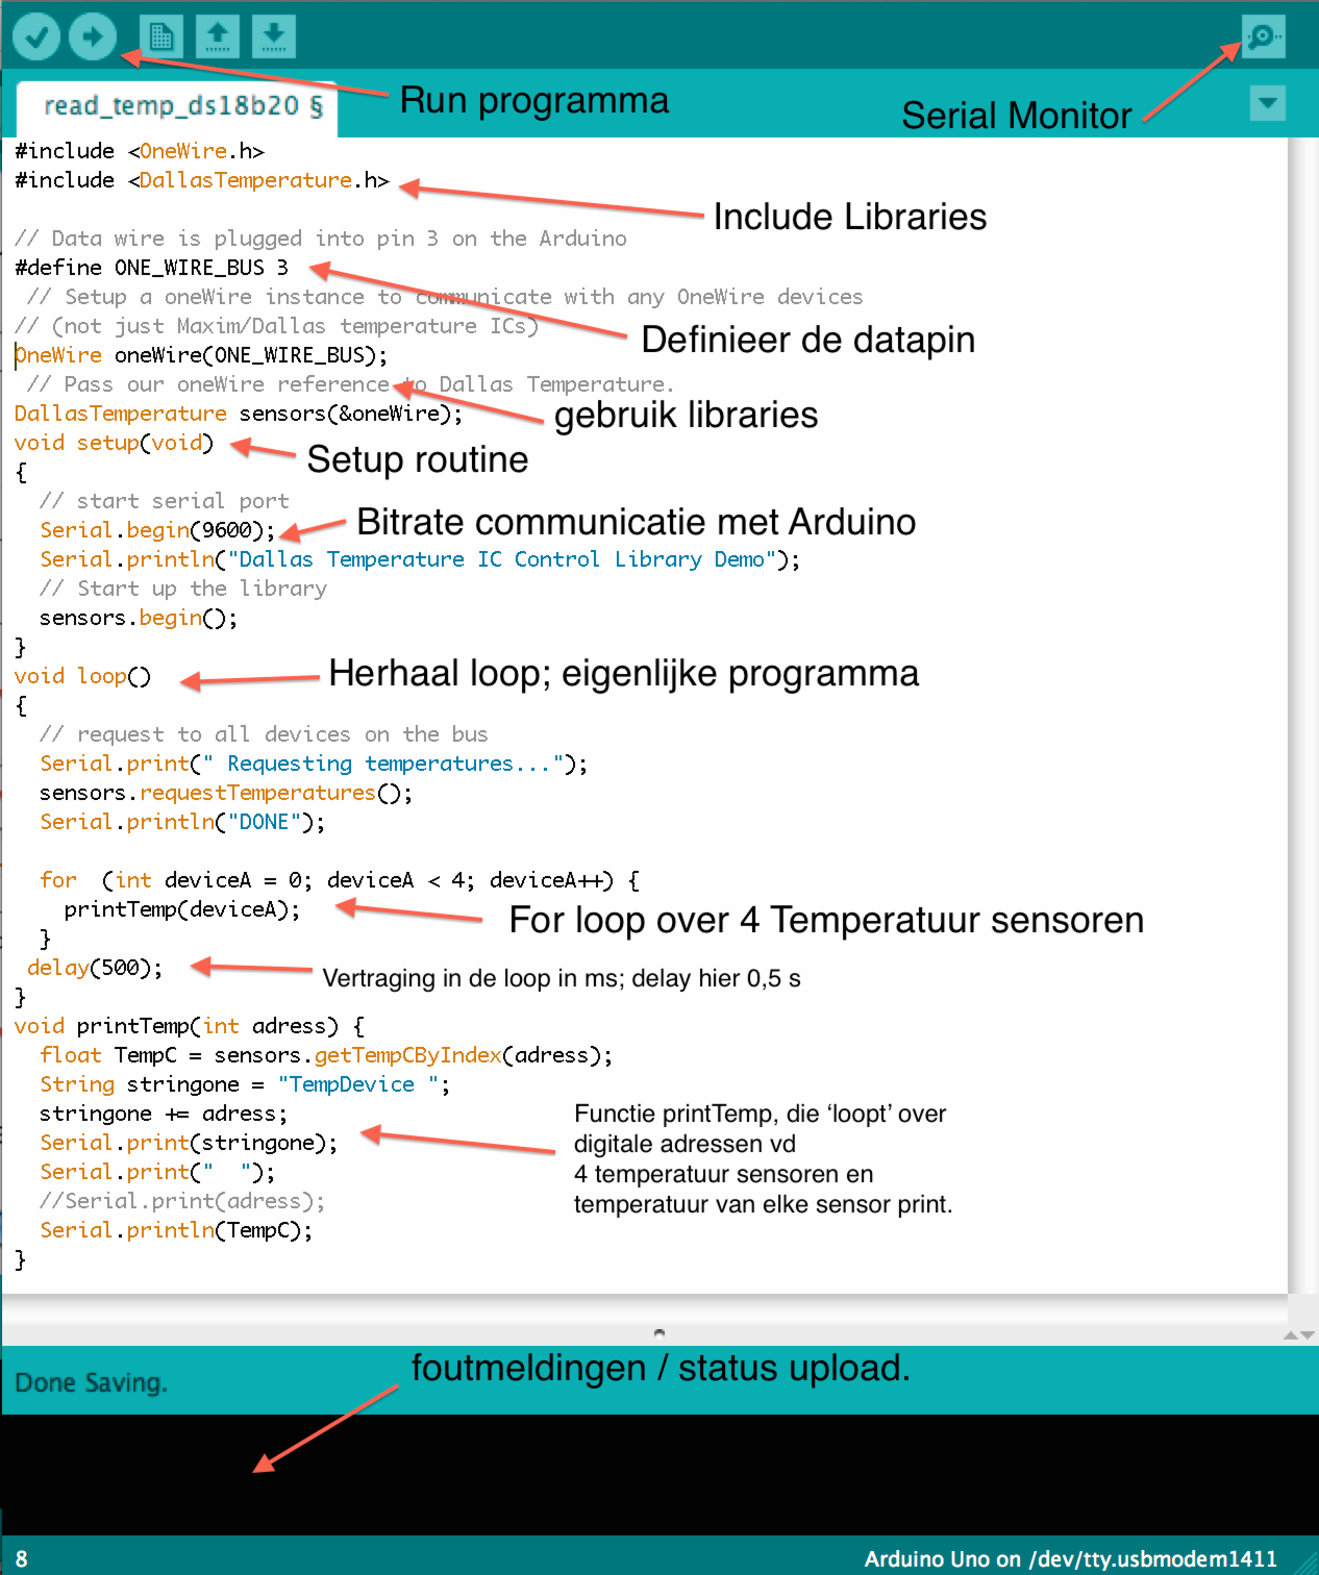
\includegraphics[scale=0.6]{Arduino_program_uitleg_3}
    \caption{Arduino Software, de belangrijkste onderdelen van een 
    programma uitgelegd. Eerst worden libraries ingeladen met 
    met het include statement. Dan wordt de datapin gedefinieerd.
    Libraries worden aangeroepen. In \emph{void setup} definieert u variabelen, 
    kunt u libraries starten. De \emph{void setup} wordt één keer uitgevoerd. 
    \emph{Void loop} is het eigenlijke programma wat continue herhaalt wordt. 
    Als laatste ziet u een zelf gedefinieerde functie (printTemp), die binnen 
    de \emph{void loop} aangeroepen wordt.}
   \label{fig:Arduino_program_uitleg_3}
\end{figure}


\section{Sensoren}

\subsection{Inleiding}

Bij dit weerstation gaan we een aantal sensoren gebruiken om naast de al
beschikbare data van de \hisparc stations ook weerdata mee te nemen in
onderzoek naar correlaties van kosmische straling met weergrootheden. We
zijn ook ge\"{i}nteresseerd in de temperatuur van de detectors.
Buisman \cite{Buisman} heeft aangetoond dat de PMT van de detector gevoelig is
voor temperatuur. Om dit verschijnsel te meten plaatsen we in elke detector 
ter hoogte van de PMT een digitale temperatuursensor (DS18B20). De luchtdruk- 
en luchtvochtigheidsensor worden bij de Arduino geplaatst in een (zelf te
ontwikkelen) weerhuisje. Leerlingen kunnen dan zelf correlaties tussen
luchtdruk en aantal events onderzoeken. De luchtvochtigheid biedt weer
opties om bijvoorbeeld het dauwpunt uit te rekenen. Hieronder worden de
verschillende sensoren kort toegelicht en uitgelegd hoe ze uit te lezen
zijn met de Arduino software. 


\subsection{Temperatuursensor}

Om de temperatuur van de detectoren te meten gebruiken we 2 of 4
dezelfde temperatuursensoren (DS18B20). Om de sensor te laten werken is
het belangrijk om de `pootjes' van de sensor op de juiste manier aan te
sluiten. Deze sensor kan geaard worden op twee van de drie pootjes en
wordt gevoed en uitgelezen op het pootje S (signal). Het pootje S
wisselt per uitvoering. Onze versie (`Keyes') heeft het `Signal' pootje
rechts,  zie \figref{fig:DS18B20_A_2}. Bij uw sensor kan dit anders zijn.
Raadpleeg in dat geval de datasheet van de sensor of inspecteer de
inscripties bij de pootjes van de sensor.

\paragraph{Aansluiten en meten met de temperatuursensor}

Om de digitale temperatuursensor te gebruiken is een schakeling nodig
zoals in \figref{fig:DS18B20_schakeling} is getekend. De ground en de
voedingspin zijn beide verbonden met de ground van de Arduino. Het
Signal of data pootje is via een \SI{4.7}{\kilo\ohm} weerstand verbonden
met de \SI{5}{\volt}. Over de dezelfde draad gaat én de voeding én het
signaal. Om het geheel te laten werken hebben we echter wel twee
libraries nodig, om de temperatuursensor aan te sturen. De eerste
library \emph{OneWire} moet gedownload worden en zorgt ervoor dat
meerdere signalen over één digitale ingang uitgelezen kunnen worden. U
vindt \emph{OneWire} hier:
\url{http://playground.arduino.cc/Learning/OneWire}. Download ook de
library: \emph{DallasTemperature}. Die vindt U hier:
\url{http://milesburton.com/Main_Page?title=
Dallas_Temperature_Control_Library}

Het verdient aanbeveling om na het aansluiten van de temperatuursensoren
zoals in \figref{fig:DS18B20_schakeling}, uit de map \emph{OneWire /
example} het voorbeeld programma: \emph{DS18x20\_Temperature} uit te
voeren. Het programma zoekt dan naar de adressen van de aangesloten
temperatuursensoren. Als er geen adressen gevonden worden dan zijn de
temperatuursensoren foutief aangesloten. Verdere uitleg over het
voorbeeldprogramma staat op de volgende site:
\url{https://www.pjrc.com/teensy/td_libs_OneWire.html}.

Als alle temperatuursensoren aangesloten zijn, de libraries
ge\"{i}nstalleerd en getest, dan kunnen de temperatuursensoren
uitgelezen worden. Met de volgende code kunnen de sensoren uitgelezen
worden:


\begin{minted}{c}
#include <OneWire.h>
#include <DallasTemperature.h>
 
    // Data wire is plugged into Digital pin 3 on the Arduino
#define ONE_WIRE_BUS 3
 
    // Lib: OneWire is nodig om contact maken met ingang D3. 
OneWire oneWire(ONE_WIRE_BUS);
 
    // oneWire reference naar Lib:  Dallas Temperature.
DallasTemperature sensors(&oneWire);
 
void setup(void)
{
  // start serial port
  Serial.begin(9600);
  
  // Start up the library
  sensors.begin();  
}
void loop()
{ 
    // request to all devices on the bus
  Serial.print(" Requesting temperatures...");
  sensors.requestTemperatures(); 
  Serial.println("DONE");
  
    //  Deze code kun je gebruiken om per temperatuursensor uit te lezen.
    //  met de functie getTempCByIndex( ) kun je de gewenste sensor uit lezen.
    //  Temperatuursensor 1 krijgt index waarde 0.    

    //  Serial.print("TempDevice 1:");
    //  Serial.println(sensors.getTempCByIndex(0)); 
    //  Serial.print("TempDevice 2 :");
    //  Serial.println(sensors.getTempCByIndex(1));
    //  Serial.print("TempDevice 3 :");
    //  Serial.println(sensors.getTempCByIndex(2));
    //  Serial.print("TempDevice 4 :");
    //  Serial.println(sensors.getTempCByIndex(3));  


    //  Of een for-loop om code te sparen.  Doet hetzelfde als de code hierboven. 
    //  Hier < 4 omdat er 4 temperatuursensoren aangesloten zijn.
  for  (int deviceA = 0; deviceA < 4; deviceA++) {
    printTemp(deviceA);
  }
 delay(500);
}

void printTemp(int adress) {  
  float TempC = sensors.getTempCByIndex(adress);
  String stringone = "TempDevice ";
  stringone += adress;
  Serial.print(stringone);
  Serial.print("  ");
  //Serial.print(adress);
  Serial.println(TempC);  
}
\end{minted}


\begin{figure}
    \centering
    \subfloat[]{
        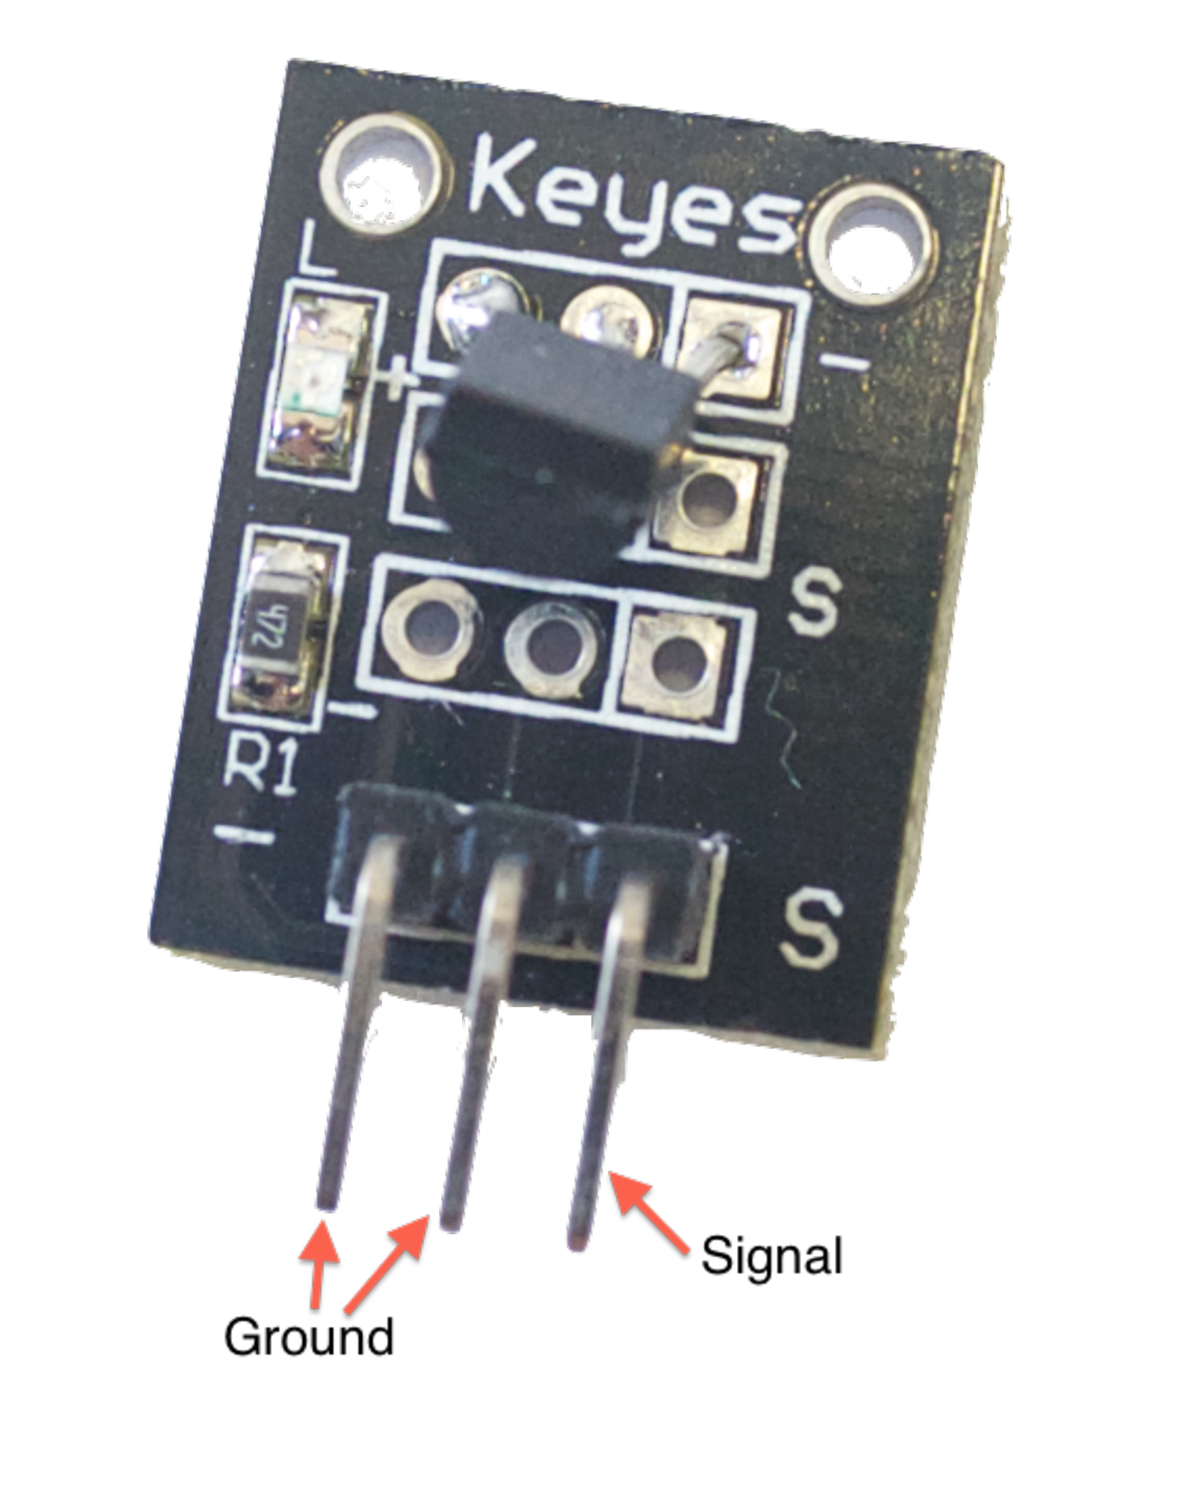
\includegraphics[width=.3\linewidth]{DS18B20_A_2}
        \label{fig:DS18B20_A_2}}
    \hfill
    \subfloat[]{
        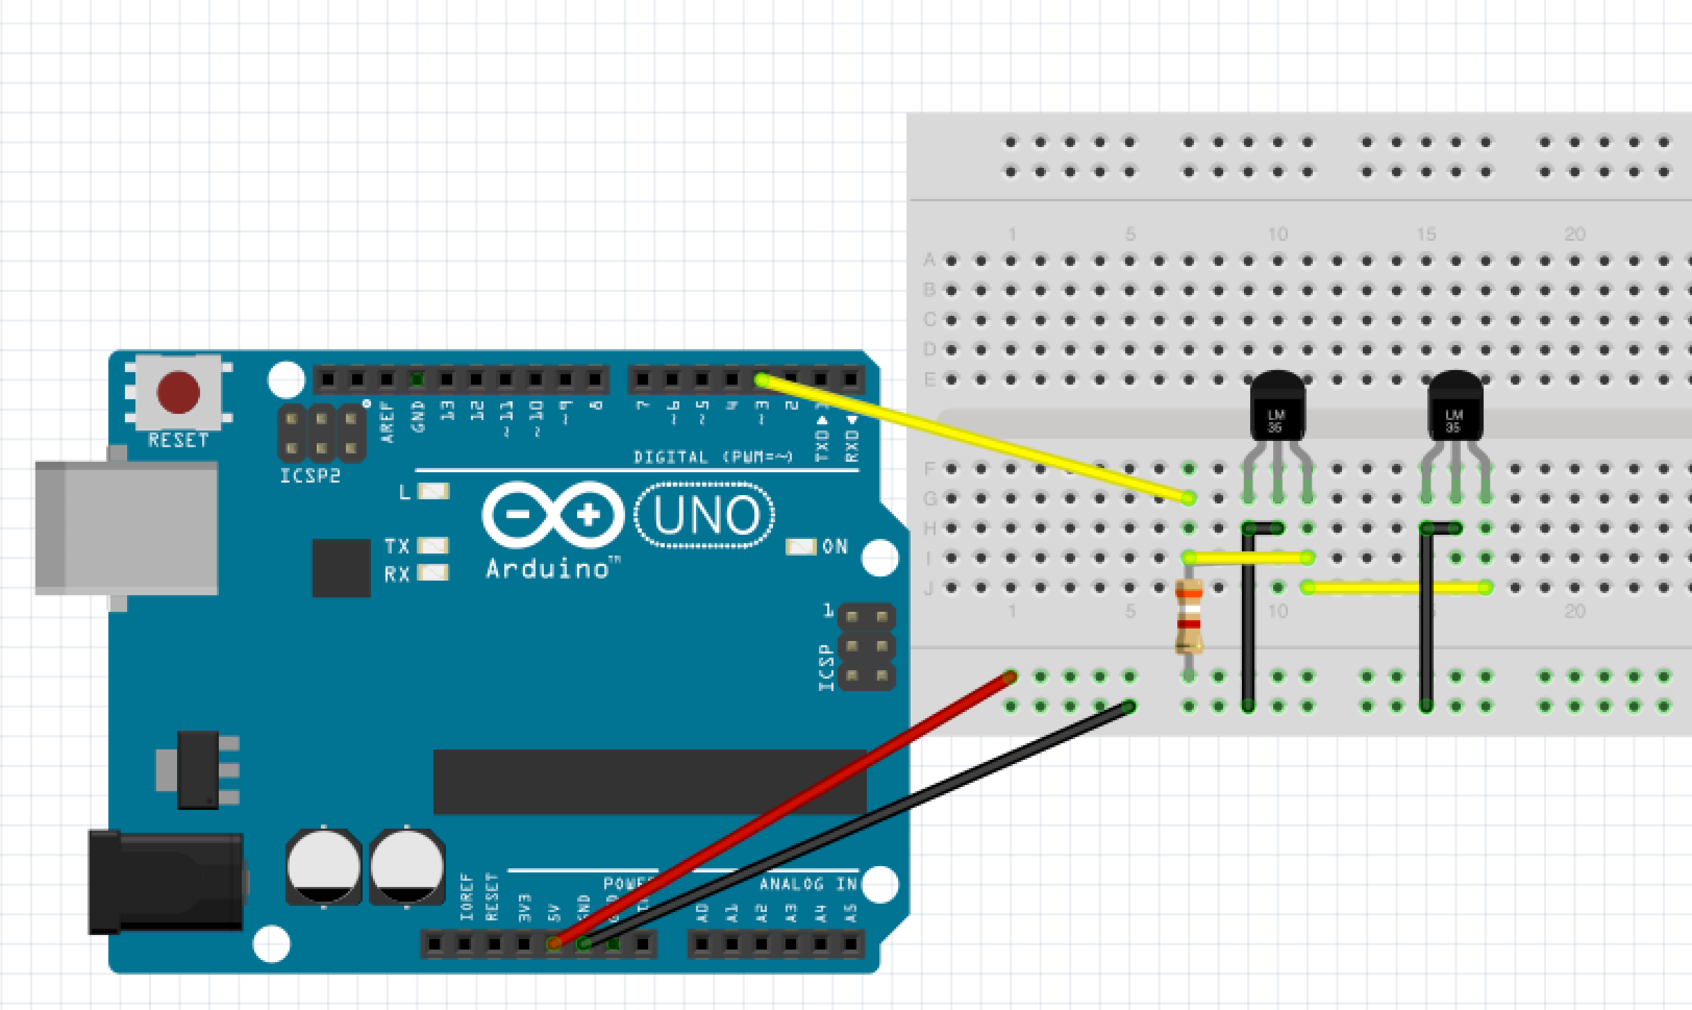
\includegraphics[width=.6\linewidth]{DS18B20_schakeling}
        \label{fig:DS18B20_schakeling}}
    \caption{De DS18B20 temperatuursensor los en in een schakeling. De gele draad 
    is zowel voeding voor de sensor als transmissie van het signaal. De zwarte 
    draad zorgt voor aarding van zowel het linker als midden pootje, dus deze 
    kan doorverbonden worden.
    Bij het testen van deze schakeling blijkt dat grotere lengte van de gele draad 
    geen signaalverlies tot gevolg heeft.}
\end{figure}

\subsection{Luchtdruksensor}

De luchtdruk gaan we met de luchtdruksensor (BMP085), die zowel luchtdruk als 
temperatuur kan meten. De data wordt verwerkt door de ingangen A4 en A5 van 
de Arduino.

\paragraph{Aansluiten en meten met de luchtdruksensor}

Zoals in \figref{fig:BMP085_A_1} te zien is heeft de luchtdruksensor 6
aansluitpootjes, waarvan wij er 4 nodig hebben. De voeding is
\SI{3.3}{\volt}, de ground van de luchtdruksensor sluiten we weer aan op
de ground van de Arduino. De luchtdruksensor is een zogenaamd $I^{2}$C
device, dat betekent dat de twee overige aansluitingen een datalijn
(SDA) en een seriële clock (SCL) zijn. Om te communiceren met de
Arduino zijn een library voor de sensor nodig en een standaard library
van Arduino om $I^{2}$C data te verwerken, namelijk \emph{Wire.h}. De BMP085
library is op verschillende plekken te downloaden, van verschillende
fabrikanten. Wij hebben de volgende (open source) library gebruikt
\emph{https://code.google.com/p/bmp085driver/} Pak deze library uit of
installeer het zip bestand van de library in een keer in Arduino via \emph{Sketch /
Import Library... / Add library} ( Arduino herkent namelijk ook \emph{zip} - bestanden).

Als de sensor is aangesloten volgens \figref{fig:Arduino_BMP_schakeling}
kan met een example programma uit de library getest worden of de sensor
werkt. In de library kan met de luchtdruk waarde ook de hoogte worden
uitgerekend, maar dan moet echter de druk op zeeniveau ook bekend zijn
en meegegeven worden. Omdat het weerstation waarschijnlijk een vaste plek
krijgt is het uitrekenen van de hoogte niet nodig en deze programma
regels kunnen verwijderd worden.

\begin{figure}
    \centering
    \subfloat[]{
        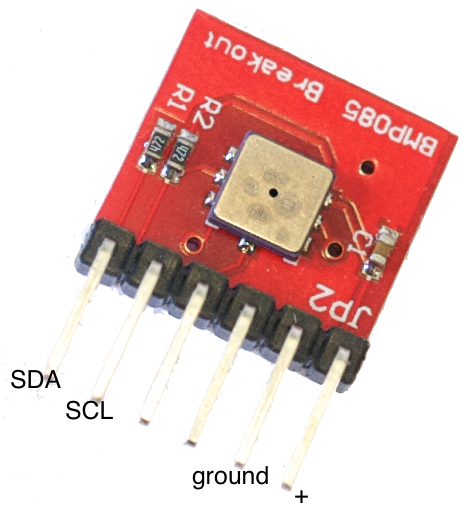
\includegraphics[width=.3\linewidth]{BMP085_A_1}
        \label{fig:BMP085_A_1}}
    \hfill
    \subfloat[]{
        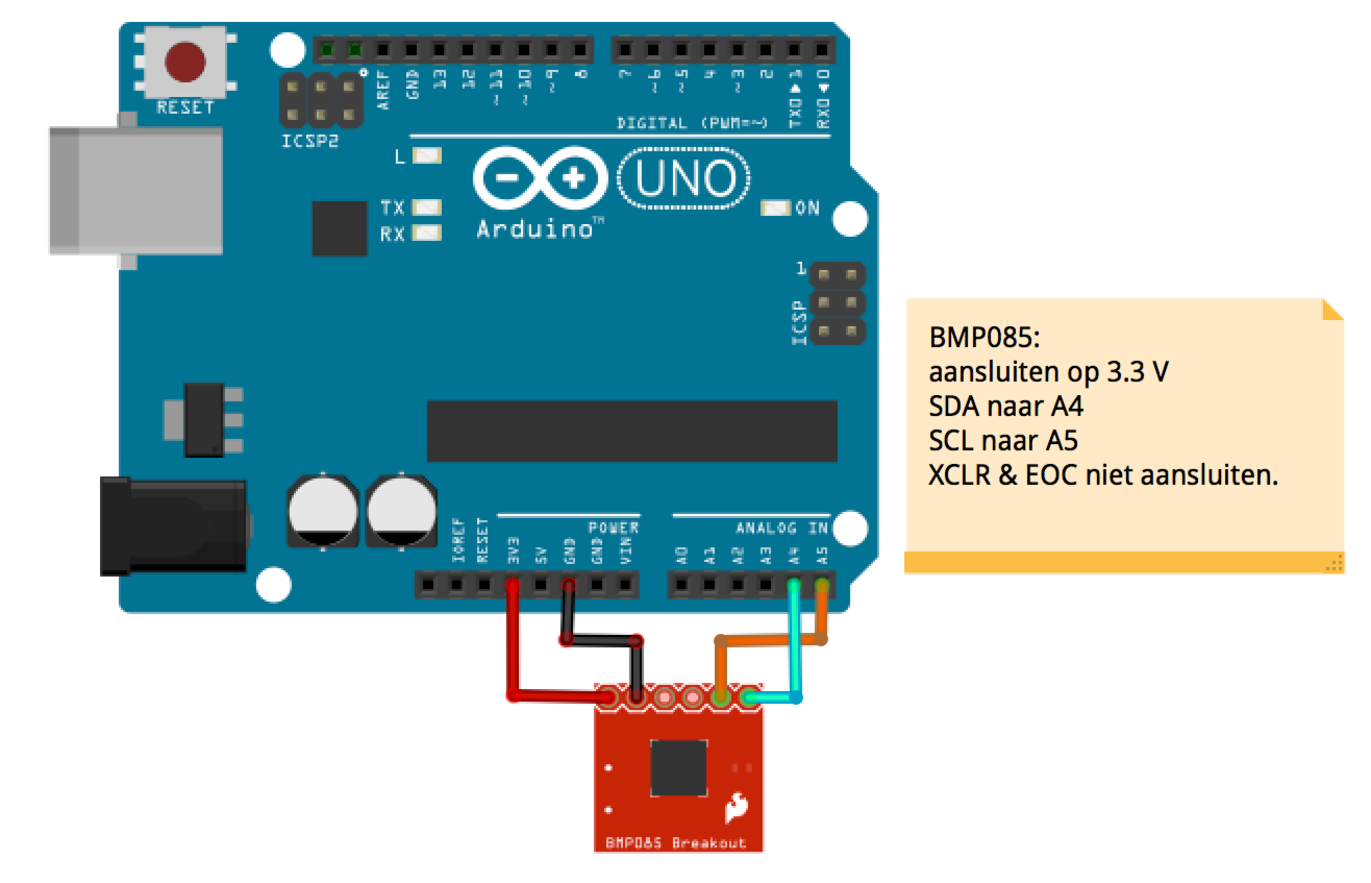
\includegraphics[width=.6\linewidth]{Arduino_BMP_schakeling}
        \label{fig:Arduino_BMP_schakeling}}
    \caption{De BMP085 los en in een schakeling. De voeding is \SI{3.3}{\volt} 
    en de data wordt via een seri\"{e}le data en clock lijn uitgelezen op A4 en A5.}
\end{figure}



\subsection{Luchtvochtigheidssensor}

De (relatieve-) luchtvochtigheid gaan we meten met de
luchtvochtigheidssensor (DHT22 of DHT11), deze sensoren kunnen ook
temperatuur meten. Wij hebben gekozen voor de iets duurdere DHT22, omdat
die nauwkeuriger is, een relatieve luchtvochtigheidsbereik van
\SIrange{0}{100}{\percent}en een temperatuurbereik heeft van
\SIrange{-40}{125}{\degreeCelsius}. De DHT11 heeft een bereik 
van \SIrange{0}{80}{\percent}, temperatuurbereik van \SIrange{0}{50}{\degreeCelsius} 
en een nauwkeurigheid van \SI{5}{\percent}.

\paragraph{Aansluiten en meten met de luchtvochtigheidssensor}

De luchtvochtigheidssensor heeft 4 pinnen, waarvan we er 3 gebruiken. De
linkerpin is de voeding \SI{5.0}{\volt}, de 2e pin van links is de
datapin, die wordt via een weerstand van \SI{10}{\kilo\ohm} verbonden
aan digitale ingang 2 van de Arduino. De derde pin van links is niet in
gebruik. De rechter pin is de ground. Zie \figref{fig:DHT22_A_3}. We hebben
wederom een library nodig om de DHT werkend te krijgen in de Arduino
software. De library voor DHT22 of DHT11 is te downloaden van
\url{http://playground.arduino.cc/Main/DHTLib}, klik daar op
\emph{latest version on github}. Als de sensor aangesloten is volgens
\figref{fig:Arduino_DHT_schakeling}, kan weer een example geprobeerd
worden die bij de library geleverd wordt.

\begin{figure}
    \centering
    \subfloat[]{
        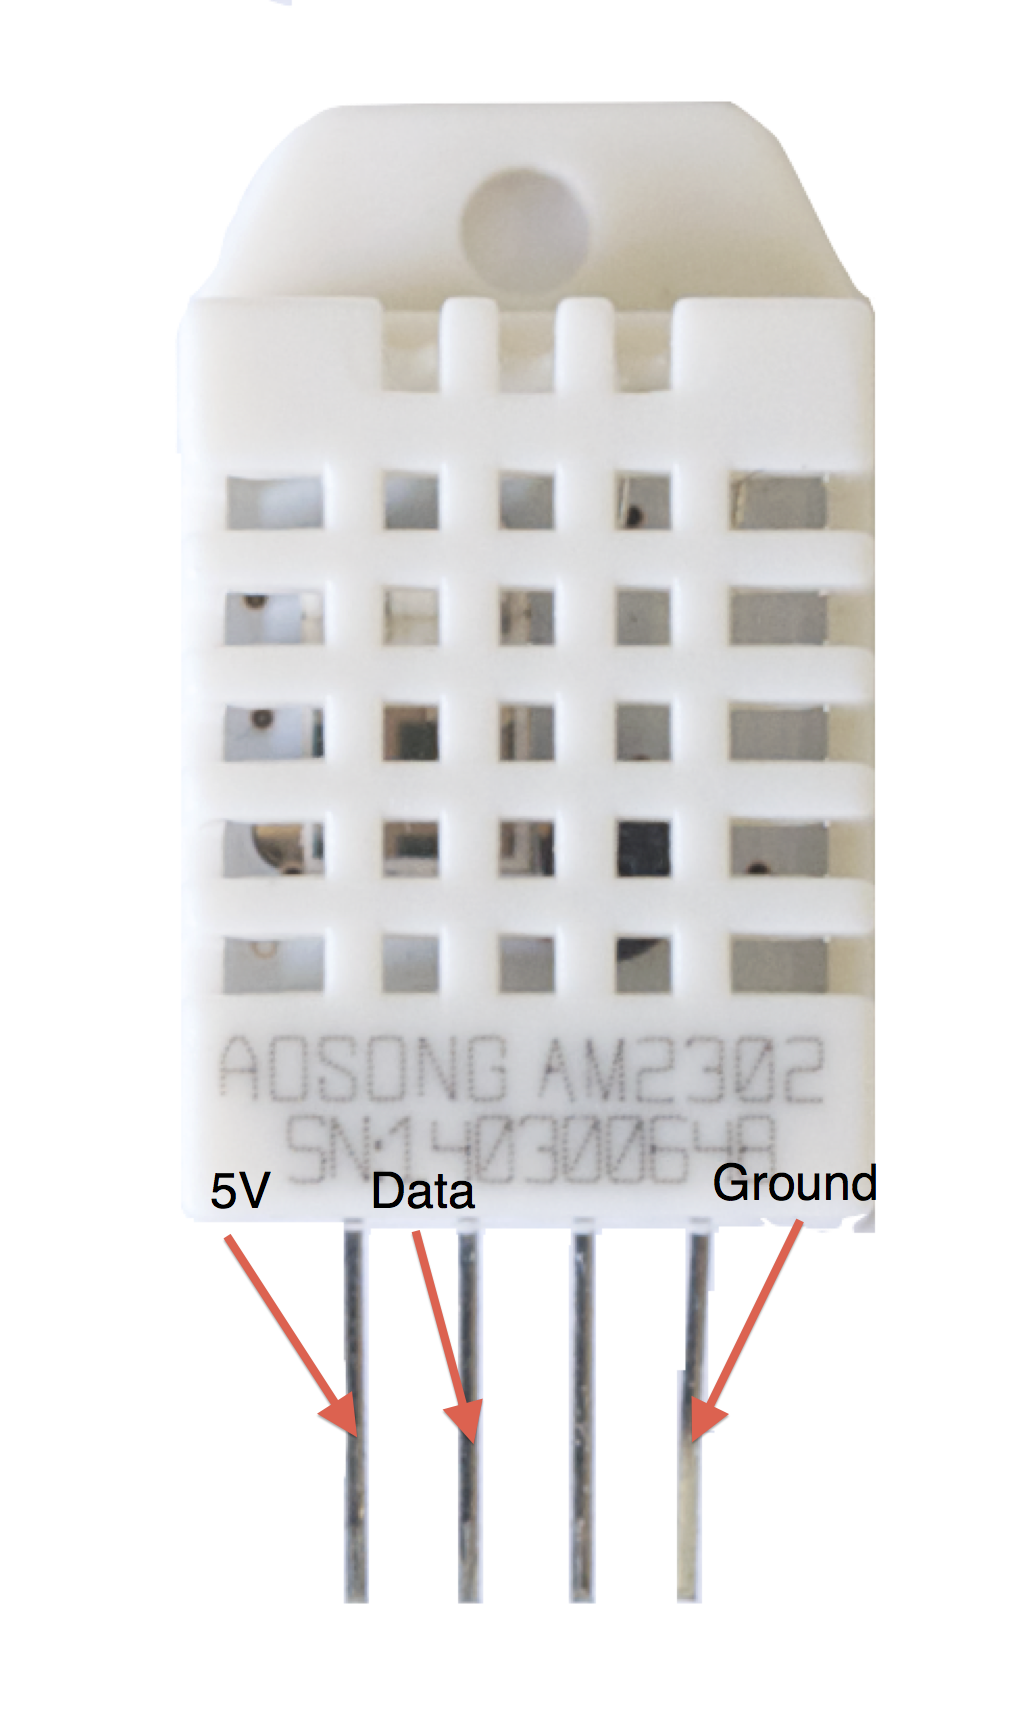
\includegraphics[width=.3\linewidth]{DHT22_A_3}
        \label{fig:DHT22_A_3}}
    \hfill
    \subfloat[]{
        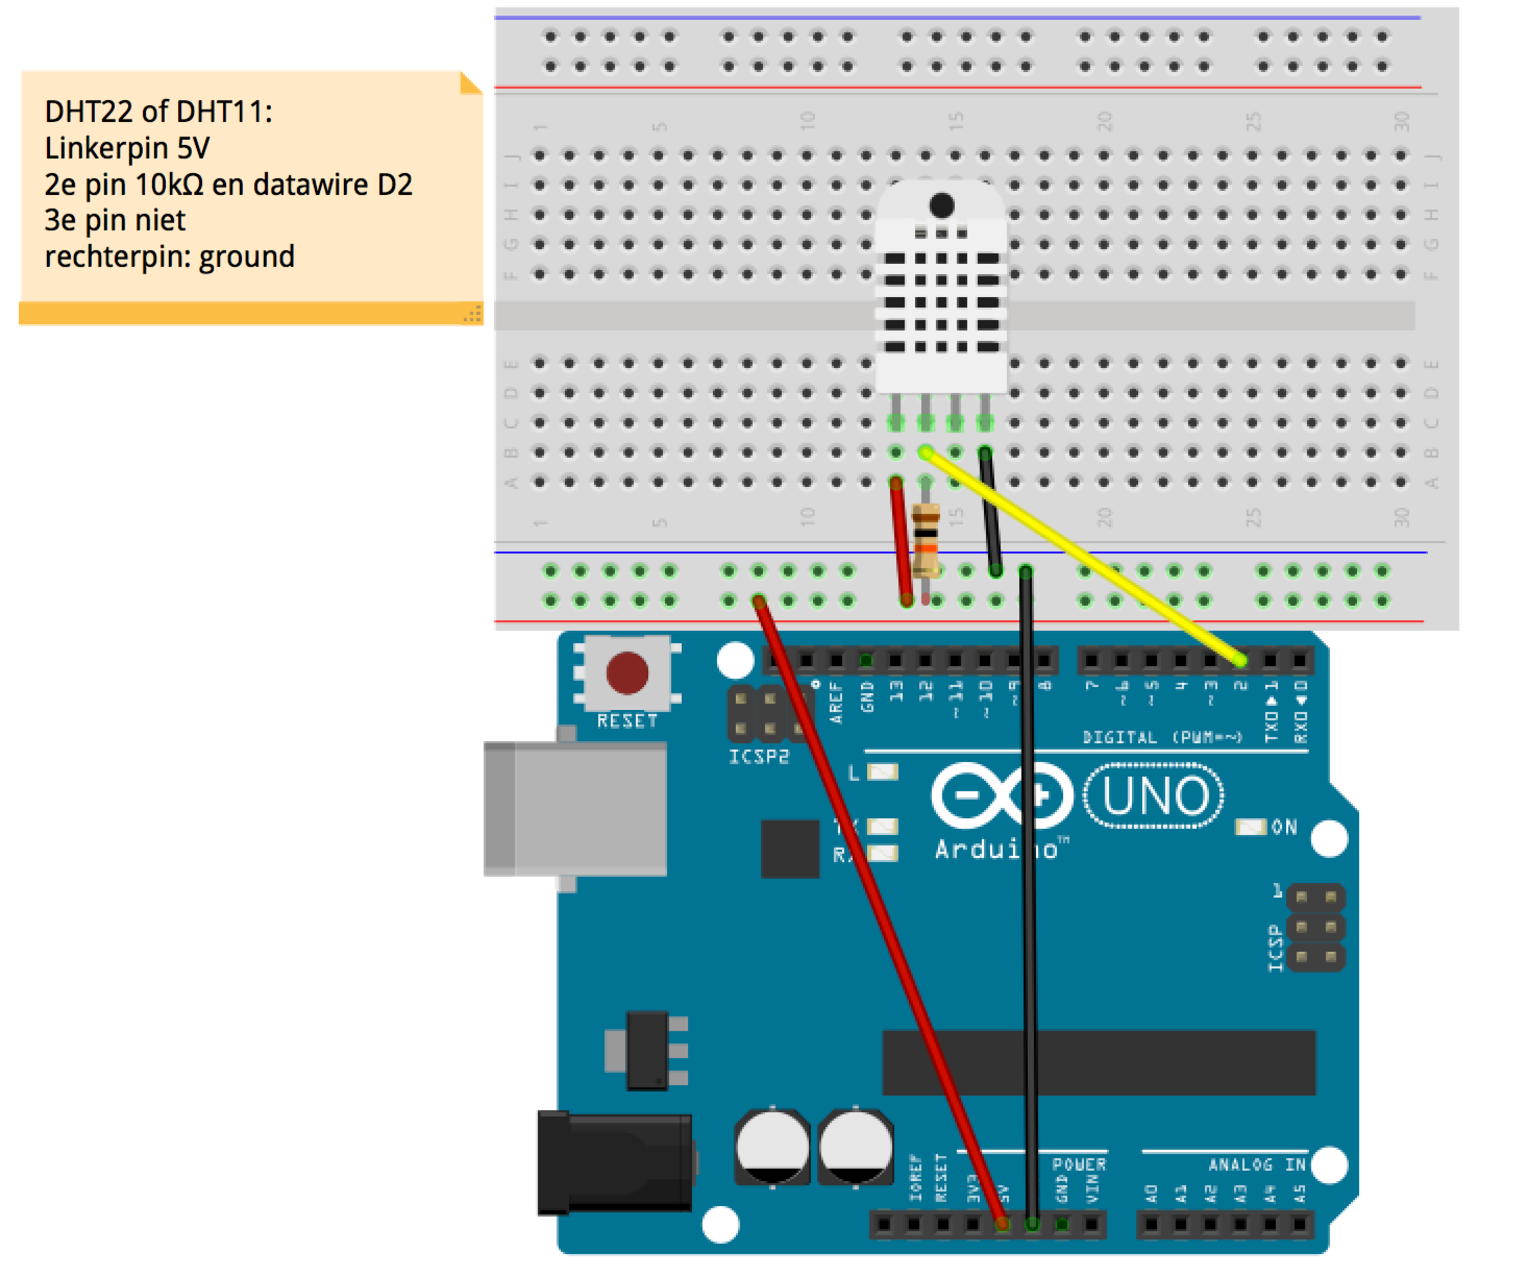
\includegraphics[width=.6\linewidth]{Arduino_DHT_schakeling}
        \label{fig:Arduino_DHT_schakeling}}
    \caption{De DHT los en in een schakeling. De voeding is \SI{5.0}{\volt}. 
    Naar de datapin zit een weerstand van \SI{10}{\kilo\ohm}. Zowel de
    temperatuur als de relatieve luchtvochtigheid worden uitgelezen via
    een ingang.}
\end{figure}

\subsection{Weerstation}

Nu we alle sensoren afzonderlijk hebben getest,kunnen we de sensoren
gaan combineren en ook het programma schrijven wat alle sensoren in een
keer netjes uitleest en de waarden netjes print. Deze waarden kunnen we
dan samen met een datum en tijd functie printen of wegschrijven naar een
textfile of spreadsheetprogramma.

In \figref{fig:Arduino_weerstation_schakeling} zien we alle sensoren (op
een breadboard) aangesloten op een Arduino. We kunnen nu meten met het weerstation, 
we hebben echter nog wel een vaste verbinding nodig. In de hieropvolgende 
handleiding gaan we het weerstation draadloos maken.  
In de volgende handleiding 'weerstation data' lezen we deze data uit van 
de Arduino en sturen we dat naar de \hisparc database.




\begin{figure}
    \centering
    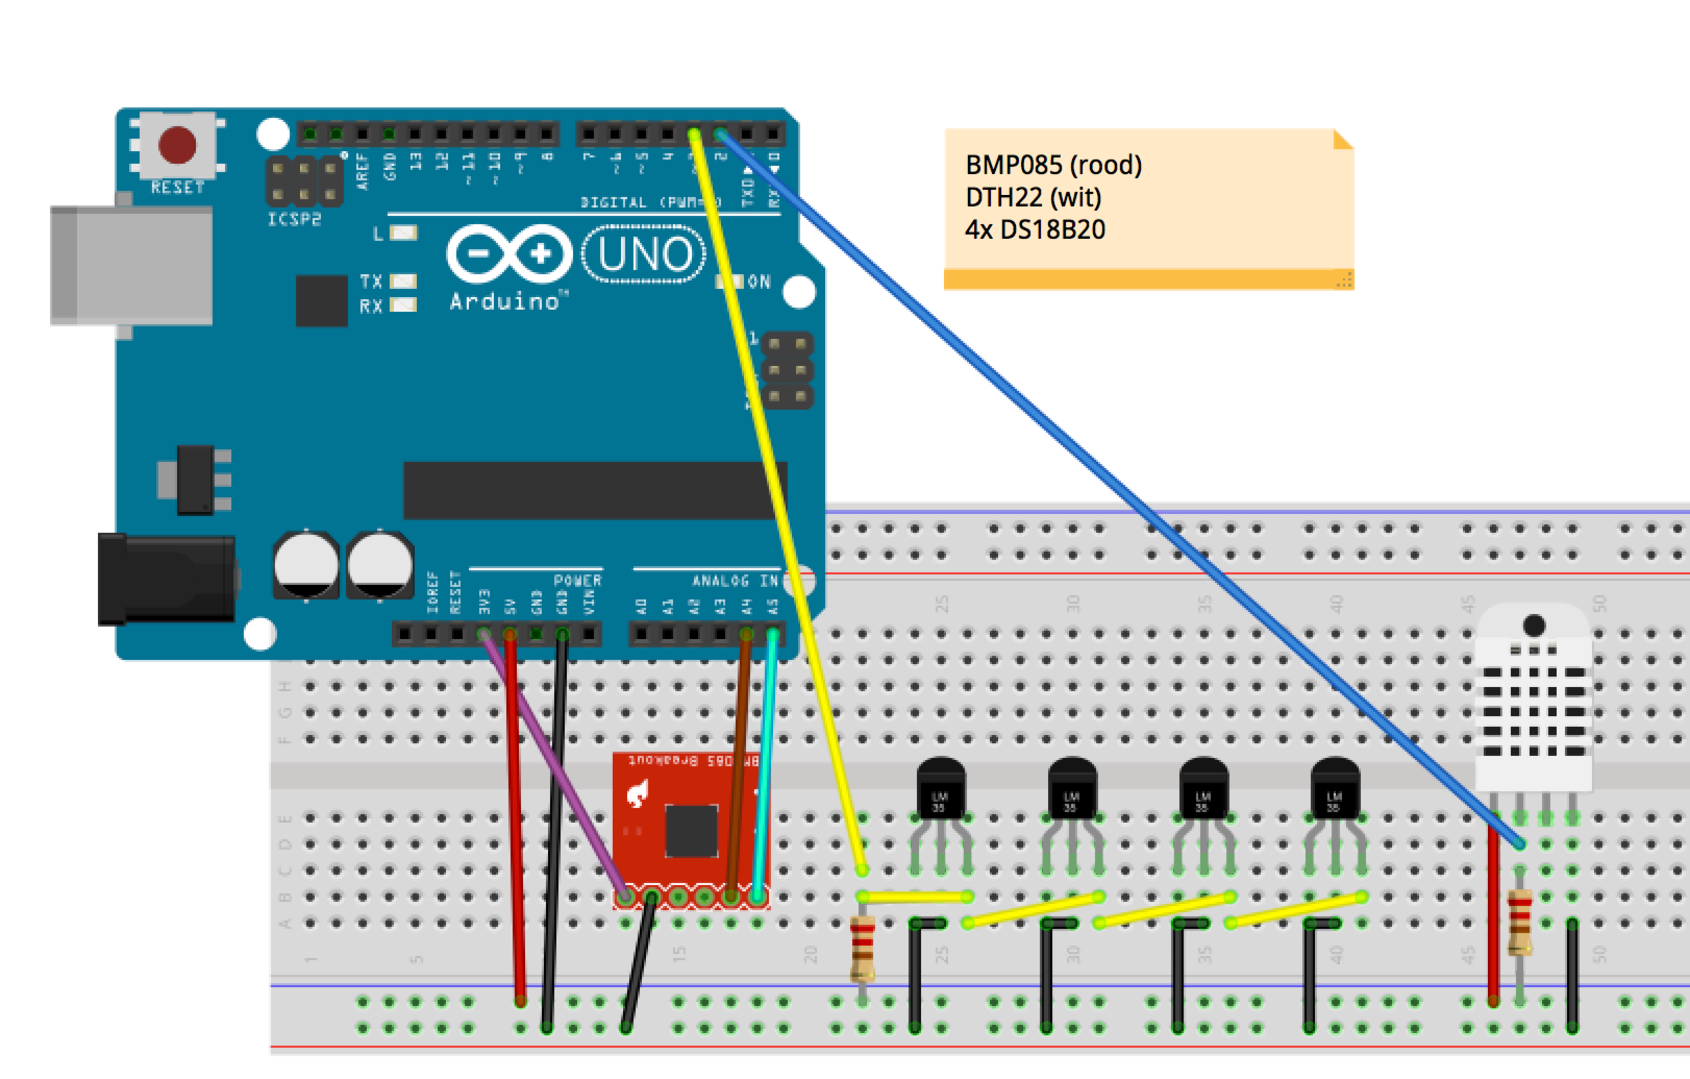
\includegraphics[scale=0.5]{Arduino_weerstation_schakeling}
    \caption{Alle sensoren aangesloten op de Arduino}
   \label{fig:Arduino_weerstation_schakeling}
\end{figure}


\section{FAQ}

Bij het werken met Arduino en de sensoren zijn er een aantal zaken die vaak mis
gaan. De meest voorkomende worden hieronder opgesomd en beantwoord.

\begin{itemize} 
    \item \emph{Arduino wil niet uploaden.} Zorg dat het
    juiste Arduino bordje is geselecteerd, dit stel je in, in de Arduino
    software bij \emph{Tools/Board} vink daar het juiste Arduino bordje aan.
    \item \emph{Foutmelding bij uploaden} De juiste usb poort moet altijd
    ingesteld zijn. Vink daarom de juiste usb poort aan. De Arduino software
    vindt deze niet altijd automatisch. Zoals te zien is in
    \figref{fig:Arduino_serial}. Is de USB poort niet juist dan zie je de
    volgende foutmelding in het venster.
    \verb|avrdude: stk500_recv(): programmer is not responding|.
    \item \emph{Onjuiste data.} Zorg dat je in je Arduino code op de juiste 
    ingangen uitleest. Check of je de juiste pinnen van de Arduino hebt aangesloten
    de uitgangen van de sensoren en of deze matchen met de gebruikte waarden in de
    code.
    \item \emph{Rare meetwaarden in serial
    monitor} Als de meetwaarden van de sensoren niet veranderen of de hele
    tijd dezelfde waarden geven, dan moet de schakeling gecontroleerd
    worden. Het verdient aanbeveling om de schakeling helemaal af te breken
    en opnieuw te maken.
    \item \emph{Andere foutmeldingen} Check the troubleshooter van Arduino: 
    \url{http://arduino.cc/en/guide/troubleshooting#toc1} 
    
\end{itemize}

\begin{thebibliography}{9}
    \bibitem{Buisman}
        H. Buisman, \emph{\hisparc Experiment: Lichtopbrengst en temperatuur}, 
        Lio jaarverslag 2011
\end{thebibliography}


\end{document}
